\section{Componentes do Beaglebone Black}
\label{ch:bbb_components}

No capítulo \ref{ch:introduction} foi introduzido o Beaglebone Black como um mini computador de arquitetura ARM. Esta seção irá mostrar os componentes da placa e os integrados ao SOC Sitara AM335x. Na figura \ref{figura:bbb_components} tem-se uma foto de frente e verso da placa de circuito impresso do BBB, identificando os componentes, e na tabela \ref{tab:bbb_components} identifica a função de cada componente na placa. Para complementar na figura \ref{figura:bbb_soc} mostra os componentes integrados ao SOC Sitara AM3358A, este último disponível na \emph{rev.3} deste produto.

\begin{table}[h]
	\centering
	\begin{tabular}[c]{ccm{10cm}}
		No.&Componente&Função\\ \hline
		1&Sitara AM335x&SOC do BBB contendo diversos componentes integrados incluindo a CPU, GPU e PRU.\\
		2&HDMI Framer&Converte o controlador de LCD do AM335x.\\
		3&Memória RAM&512MB DDR3.\\
		4&eMMC&4GB de memória de armazenamento interna.\\
		5&TPS65217C&Regulador de potência sofisticado com 4 reguladores de tensão LDO controlado por I2C\\
		6&Ethernet PHY&Conecta o processador ARM a conexão física RJ45 com a velocidade de 100Mbit para enviar e 10Mbit para receber.\\
		7&7x LEDs&\emph{Power} LED (azul), 4 \emph{user} LEDs e 2 LEDs (amarelo = dados enviados/ verde = dados recebidos).\\
		8&\emph{Push Buttons}&Liga/Desliga (\emph{Power}), \emph{Reset Button} e \emph{Boot Switch}. Este último seleciona se o deve ser feito \emph{boot} do eMMC ou do cartão micro SD.\\
		9&Micro HDMI&Para conectar em monitores de até 1280x1024@60Hz ou 1920x1080@24Hz.\\
		10&Ethernet RJ45&Conector RJ45.\\
		11&5V DC& \emph{Jack} de 5mm para usar o BBB sem precisar alimentar com o cabo USB.\\
		12&\emph{Slot} micro SD& \emph{Slot} para cartão micro SD;\\
		13&\emph{Serial Debug}&Conector de 6 pinos para acessar o terminal através da conexão serial (UART0).\\
		14&USB 2.0 \emph{Client}&Conector mini-USB 2.0 utilizado para conectar o BBB ao computador.\\
		15&USB 2.0 \emph{Host}&Conector USB-A 2.0 para conectar os periféricos do BBB, como \emph{webcams}, \emph{mouse}, teclado e outros. Pode-se utilizar um \emph{hub} USB para conectar mais de um periférico.\\
		16\&17&Expansões P8 e P9&Soquete de pinos de extensão P8 e P9. Cada soquete tem 2x23 pinos totalizando 92 pinos no total.\\
		18&JTAG&Espaço para conector JTAG, bastante utilizado em testes de placas de circuito impresso. Porém, necessita de \emph{software} e \emph{hardware} adicional.\\
		19&Conector de bateria&É possível soldar estes 4 pinos para adicionar um conector de bateria a placa.\\
		\hline
	\end{tabular}
	\caption{Relação dos componentes do BBB de acordo com a figura \ref{figura:bbb_components} \cite{derekbbb}.}
	\label{tab:bbb_components}
\end{table}

\begin{figure}
	\centering
	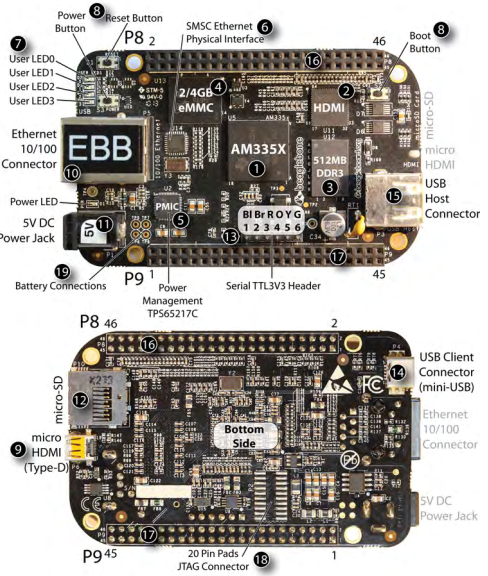
\includegraphics[width=0.6\textwidth]{figuras/bbb_componentes.png}
	\caption{O Beaglebone Black e seus componentes.\cite{derekbbb}}
	\label{figura:bbb_components}
\end{figure}

\begin{figure}
	\centering
	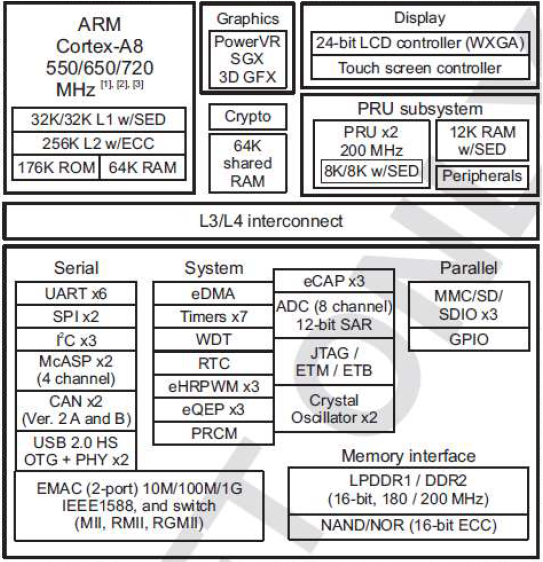
\includegraphics[width=0.6\textwidth]{figuras/bbb_soc.png}
	\caption{Diagrama do Satira AM3358A.\cite{bbbdatasheet}}
	\label{figura:bbb_soc}
\end{figure}

\section{Beaglebone Black e o Linux Embarcado}
\label{ch:bbb_elinux}

Como foi dito nos capítulos anteriores, o Beaglebone Black é um minicomputador completo que é capaz de rodar diversas distribuições de \emph{E-Linux}, Android e outros sistemas operacionais portados para arquitetura ARM. Atualmente a comunidade do Beaglebone portou apenas Android e algumas distribuições Linux, como Debian, Ubuntu, Ångström e Arch Linux. As primeiras versões do Beaglebone Black, mais especificamente as revisões 1 e 2, vinham com Ångström instalado por padrão, uma distribuição linux criada exclusivamente para sistemas embarcados, \emph{tablets}, PDAs, \emph{set top boxes}, roteadores e outros dispositivos baseados na arquitetura ARM \cite{sitebbbang}.

Entretanto, uma parte dos usuários preferiam instalar outra distribuição, como o Ubuntu, pois esta parcela de usuários na maioria das vezes não tinha muita convivência com o Linux e o fato de trabalhar numa distribuição que não tem suas raízes comuns as distrbuições populares para \emph{desktop} tornava o sistema menos amigável. Percebendo a popularidade de tutoriais ensinando como trocar de distribuição, a Texas passou a incluir a distribuição Debian a partir da revisão 3 do Beaglebone Black, lançada em 2014, e revisão mais recente desta placa, além disso, na revisão 3 houve um aumento na memória interna de 2GB para 4GB. Essas adições tornaram o BBB mais atraente para ser usado como computador, pois o espaço extra permitia a instalação de aplicativos para Linux como o \emph{Open Office}, reprodutores de video e editores de imagens.

A nova distribuição facilitou, também, na execução de aplicativos com interface gráfica (GUI) baseados nas \emph{frameworks} GTK+ e Qt, que são bastante populares no Linux \emph{desktop} baseados no Debian e seus derivados, como Ubuntu e Linux Mint. O uso de aplicativos gráficos é bastante comum nas \emph{E-Linux Board} para servir como interface entre o usuário e a máquina. Na figura \ref{figura:bbb_cnc} mostra o exemplo de uma máquina CNC controlada por um Beaglebone e a \emph{cape} K9 CNC I/O. Para controlar a CNC a fabricante da \emph{cape} criou um aplicativo com interface gráfica para Linux onde o usuário é capaz de visualizar o processo e interagir com a CNC.

\begin{figure}[h]
	\centering
	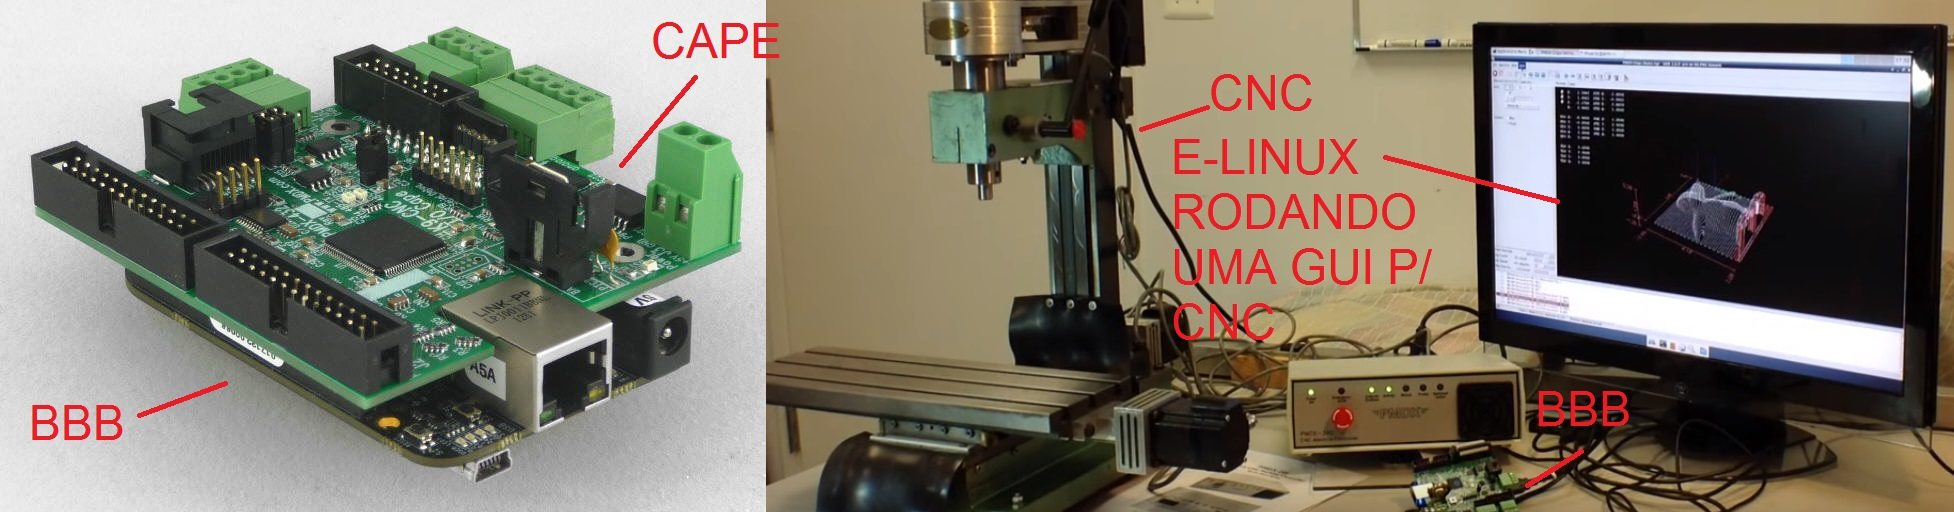
\includegraphics[width=\textwidth]{figuras/cnc_cape.JPG}
	\caption{Beaglebone controlando uma CNC e rodando uma aplicação para CNC simultaneamente.\cite{guicncbbb}}
	\label{figura:bbb_cnc}
\end{figure}

As distribuições baseadas no Debian já vem com as interfaces gráficas e pacotes relacionados instalados por padrão, incluindo aqueles necessários para executar aplicativos criados em Qt ou GTK+. Além disso, essas distribuições vem com diversos outros pacotes que são padrão para a maioria dos usuários Linux, um grande exemplo é o gerenciador de pacotes \emph{apt} que está disponível no Debian, mas não no Ångström.

\subsection{Instalando uma nova distribuição no BBB}

Na seção \ref{ch:bbb_elinux} falo-se da importância de utilizar a distribuição Debian, portanto, se o Beaglebone Black adquirido for anterior a rev.3 deve-se instalar o Debian 7.5 Wheezy, versão de 14/05/2014. Caso o Beaglebone venha uma versão do Debian superior a esta é recomendado fazer o \emph{downgrade} para a versão 7.5, principalmente, se for a versão 8 Jessie ou superior. A versão 7.5 foi projetada pensando, também, nas revisões anteriores a rev. 3, por isso ocupa um pouco menos de 2 Gb, sobrando aproximadamente 2 Gb dos 4Gb da eMMC do BBB, caso este tenha sido adquirido depois de 2014. Esse espaço extra será o suficiente para instalar novos programa, módulos e gerar grandes arquivos de dados. Uma outro motivo fazer o \emph{downgrade} é que neste trabalho e na maioria das bibliografias encontrada na literatura atualmente faz o uso desta versão do Debian, portanto pode haver procedimentos que não sejam os mesmos em versões diferentes, dificultando a reprodução dos experimentos feitos nesta monografia. 

A primeira coisa que deve ser feita para instalar uma nova distribuição é fazer o \emph{download} do sistema operacional, que pode ser baixado na página que contém as  últimas imagens pra Beaglebone Black (\emph{https://beagleboard.org/latest-images}). Caso o leitor desta monografia esteja lendo-a muito tempo depois da sua publicação existe uma alternativa no domínio oficial do Debian (\emph{https://debian.beagleboard.org/images/}), ou ainda, no site do E-Linux (\emph{http://elinux.org/Beagleboard:BeagleBoneBlack\_Debian}). No site das últimas imagens para BBB existem duas versões do Debian 7.5 de 14/05/2014. Uma delas é para utilizar o sistema operacional pelo cartão SD (\emph{without flashing the eMMC}), enquanto a outra grava o sistema operacional na eMMC (\emph{eMMC flasher}). É preferível que o sistema operacional seja instalado na memoria interna do Beaglebone, pois, além desta ter uma taxa de leitura e escrita maior que o cartão SD, ficamos com o \emph{slot} SD livre para ser utilizado em outras ocasiões.

O formato do arquivo baixado é \emph{.img.xz} que é um formato de compactação bastante comum no Linux. Caso o usuário esteja usando o Windows talvez seja necessário fazer o \emph{download} de alguma ferramenta capaz de descompactar este formato de arquivo, visto que alguns aplicativos de descompactação, como WinRar, não trabalham com este tipo de arquivo. Uma sugestão de descompactador capaz de trabalhar com este formato de compactação é o 7-Zip (Disponível em: \emph{http://www.7-zip.org/}), gratuito, \emph{open source} e sem propagandas.

Enquanto a imagem do sistema operacional está sendo baixada, deve-se fazer o \emph{download} de outro programa para gravar a imagem no cartão de memória. Uma sugestão dada pela Wiki do E-Linux é o Win32 Disk Imager (https://sourceforge.net/projects/win32diskimager/) \cite{elinuxupdatebbb}. Quando ambos os arquivos estiverem baixados, descompacte a imagem do Debian que está no formato \emph{.img.xz} e irá obter um arquivo \emph{.img}. Insira o cartão SD no leitor de cartão do seu computador. Abra o Disk Imager selecione a letra correspondente a partição do cartão de memória, selecione a imagem do Debian e clique em gravar como mostra na figura \ref{figura:update_bbb}. Irá aparecer uma caixa de mensagem explicando que esta operação pode danificar os dados no cartão, clique em \emph{yes} espere o processo ser finalizado.

\begin{figure}[h]
	\centering
	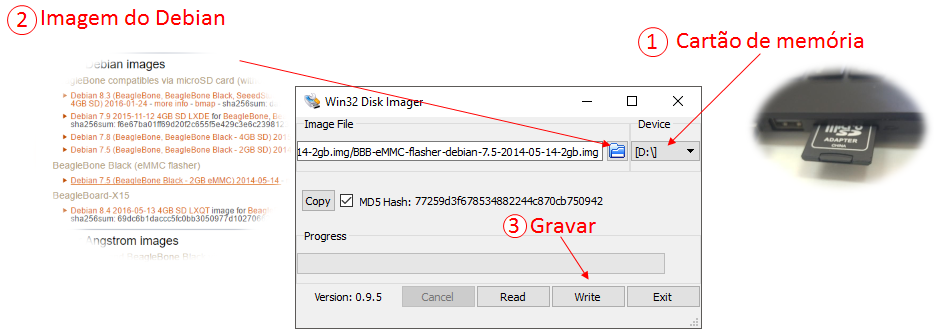
\includegraphics[width=\textwidth]{figuras/update_bbb.png}
	\caption{Gravando a imagem do Debian 7.5 de 14/05/2014 no cartão SD (Próprio Autor)}
	\label{figura:update_bbb}
\end{figure}

Depois do processo de gravação finalizar com sucesso retire o cartão SD do cartão e com o BBB ainda desligado, insira o microSD no \emph{slot} apropriado (Item 12 na figura \ref{figura:bbb_components}). Antes de ligar a placa, mantenha pressionado o \emph{Boot Switch} (Item 8 na figura \ref{figura:bbb_components}), e ainda com o botão pressionado, conecte a porta USB \emph{Client} do Beaglebone (Item 14 na figura \ref{figura:bbb_components}) e ao computador ou alguma fonte de alimentação. Depois dos \emph{User LEDs} (Item 7 na figura \ref{figura:bbb_components}) começarem a piscar solte o \emph{Boot Switch}. A partir daí, o sistema operacional será instalado na eMMC o processo dura cerca de 30 a 40 minutos, durante este tempo não desligue o Beaglebone. Quando a instalação estiver concluída os 4 \emph{User LEDs} irão se apagar. Neste momento desconecte oo cabo USB da fonte de alimentação retire o cartão SD e conecte novamente o BBB ao computador. Será montada uma partição FAT com o nome \emph{BeagleBone Getting Started} clique nela e abra o arquivo \emph{ID.txt} com o bloco de notas. Se aparecer \emph{BeagleBoard.org BeagleBone Debian Image 2014-04-23
} a atualização da Distro foi realizada com sucesso (Figura \ref{figura:check_bbb_version}).

\begin{figure}[h]
	\centering
	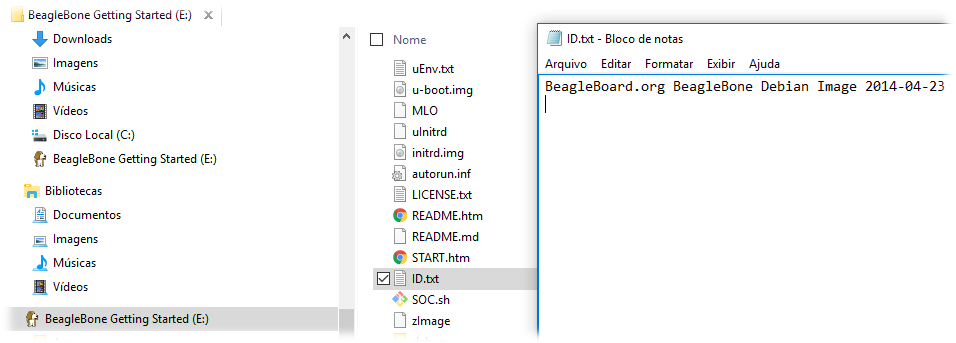
\includegraphics[width=\textwidth]{figuras/check_bbb_version.png}
	\caption{Verificando a atualização do Debian 7.5 foi instalada com sucesso. (Próprio Autor)}
	\label{figura:check_bbb_version}
\end{figure}

\subsection{Comunicando com o BeagleBone Black}

O Beaglebone Black \emph{vanilla}, ou seja, da forma como veio de fábrica, não tem nenhuma interface de interação com o usuário além de alguns \emph{push-bottons} e LEDs indicadores (Itens 7 e 8 da figura \ref{figura:bbb_components}), e isso não é o suficiente para programar ou adicionar alguma nova função a placa de desenvolvimento, a menos que o usuário use o BeagleBone ligado a um monitor, mouse e teclado. Para interagir com o \emph{board computer} sem a necessidade desses aparelhos é necessário se comunicar com o BBB através de um computador hospedeiro. Existem diversas formas de fazer esta comunicação, mas esta seção irá focar na protocolo SSH e no \emph{serial debug}, primeiro iremos falar do SSH.

Nos primórdios da informática não existia mouse, nem sistema operacional com interface gráfica, janelas e menus. Portanto, a interação homem-máquina era feita por comandos que executavam aplicativos e faziam operações, como entrar em diretórios, copiar arquivos, escrever documentos e até mesmo programar. Este tipo de interação homem-máquina ficou conhecido como linha de comando e era bastante popular em sistemas operacionais antigos, como DOS. Com o surgimento do Windows, a Microsoft passou a desestimular o uso da linha de comando para o uso em detrimento à interface de janelas, em conjunto com o \emph{mouse}. Foi a partir daí que a informática começou se popularizar. A interface de janelas era mais intuitiva e, por isso, atraiu a atenção das massas.

Com o tempo as pessoas se acostumaram com o ambiente gráfico do Windows e a linha de comando ficou em abandono, não apenas pelos seus usuários, mas também pela própria Microsoft, cujo o principal objetivo era deixar o ambiente de janelas cada vez mais rico e moderno. Por motivos de legado, a empresa de Bill Gates disponibilizou o programa $cmd.exe$ ou Prompt de Comando. Ele é um emulador do DOS onde, é possível executar boa parte das operações do antigo sistema operacional. Contudo, como não houve atualizações do DOS durante décadas, o Prompt de Comando é ultrapassado, pois as novas tecnologias foram implementadas apenas na interface gráfica, tornando-o bastante pobre em relação ao ambiente de janelas. Entretanto, isto só é verdade no Windows, seus grandes concorrentes, Linux e Mac, não abandonaram a linha de comando.

O Linux e Mac são baseados em um ancestral comum, o Unix. Por isso, sua base de arquivos e a forma de como são organizados são parecidas. Uma das principais semelhanças desses sistemas operacionais é o uso da mesma linguagem de linha de comando, o Shell. Esta linguagem, ao contrário do Prompt Comando, é bastante completa sendo capaz de fazer quase todas do sistema operacional, as vezes até mais operações que a própria interface gráfica. O programa que executa os comandos Shell é chamado de terminal.


Por muito tempo, o Linux só permitia a instalação de programas e \emph{drivers} através da linha de comando, uma tarefa um tanto complicada para usuários comuns. Isso, teoricamente, afastou as pessoas comuns deste sistema operacional, chegando ao ponto que muitos atribuírem a baixa taxa de adoção do SO por causa da ausência de uma interface gráfica tão completa quanto a do Windows. Com o tempo isso mudou e hoje o Linux permite fazer quase tudo, incluindo a instalação de \emph{drivers} e aplicativos, pela interface gráfica. Porém, é possível fazer o mesmo pela linha de comando e isso é uma vantagem enorme do Linux e Mac em relação ao Windows, o freguês pode escolher a maneira de interagir com o sistema. 

Existem algumas tarefas que são muito mais rápidas e práticas serem feitas através do terminal, embora não sejam tão intuitivas quanto. Um grande exemplo disso é a automação de tarefas, com o Shell é possível criar macros ou pequenos \emph{scripts} para automatizar tarefas chatas ou repetitivas de maneira rápida. Além disso, por utilizar apenas textos para enviar e mostrar informações, esta é uma forma de interação que consome poucos recursos da máquina. E ainda, o uso exclusivo de texto facilita o compartilhamento de artigos e tutoriais relacionados a interações com o sistema, principalmente se eles forem mais complexos, como alterar parâmetros de configurações, pois basta que o usuário abra o terminal copie os comandos do tutorial, cole e aperte \emph{Enter}. O mesmo tutorial utilizando interface gráfica necessitaria de alguns textos explicativos e capturas de tela, por isso que a maioria dos tutoriais para Linux disponíveis na internet são feitos para a linha de comando, embora seja perfeitamente possível fazer o mesmo pela interface gráfica. O lado ruim dessa prática é que o usuário leigo muitas vezes não tem noção dos processos necessários para a execução de tal tarefa e, por isso, não aprende o porquê ou como reproduzir o mesmo sem copiar e colar a sequência de comandos. Com esta prática, muitos usuários recém-chegados no Linux pensam que está é a única forma de fazer determinada tarefa, e acabam abandonando a plataforma por pensar que o Linux não foi feito para "seres humanos".

A sigla SSH significa Secure Shell, ou seja, uma forma de enviar comandos com criptografia, ou de forma segura, de uma máquina para outra. Este protocolo de comunicação foi criado, inicialmente, para facilitar o acesso remoto de máquinas dentro dos servidores \cite{derekbbb}. Para exemplificar, imagine que um engenheiro necessita instalar um novo aplicativo em um servidor a quilômetros de distância. Com o SSH o engenheiro pode iniciar uma conexão SSH entre o seu computador e uma das máquinas do servidor e escrever os comandos para a instalação do aplicativo, tudo através do terminal da sua máquina. Claro que operar a linha de comando não é uma tarefa para qualquer um, entretanto o fato do SSH ser baseado somente em texto, torna-o uma forma de comunicação que consome pouca largura de banda e fácil de ser implementada, além de trazer todas as outras vantagens que o Shell oferece em relação ao ambiente de janelas. Isso é evidente quando se compara o esforço necessário para fazer uma comunicação remota através de interface gráfica. Para que isso seja possível é necessário, no mínimo, fazer a captura da tela, mouse e teclado do computador remoto, enquanto, com SSH, só é necessário que haja a captura do teclado e o envio de alguns dados no formato de texto.

O protocolo SSH é orientado por IP (Internet Protocol), ou seja, faz parte do mesmo padrão de comunicação utilizado pela internet, também conhecido como pilha de protocolos TCP/IP. Este modelo surgiu como um projeto de comunicação do exército americano que com o tempo projeto se expandiu e tornou-se a \emph{internet} como conhecemos hoje. 

Atualmente o TCP/IP é baseado num modelo simplificado do padrão de referência da ISO (International Organization for Standardization) para sistemas de comunicação, o OSI (Open Systems Interconnectons). O modelo da ISO é baseado em 7 camadas hierárquicas. Cada camada é responsável por executar determinada função e deve ser especificada através de protocolos de comunicação. Estes, por sua vez, podem, ou não, ser compatíveis com os protocolos de outras camadas. Quando tomado em conjunto os protocolos das diferentes camadas, denominamos pilhas de protocolos. A pilha de protocolos da internet é chamada de TCP/IP. E ela é composta obrigatoriamente de 5 das 7 camadas do padrão OSI (Figura \ref{figura:osi_hierarquia}). As outras duas camadas, dependendo da aplicação, podem existir, mas são opcionais.

\begin{figure}[h]
	\centering
	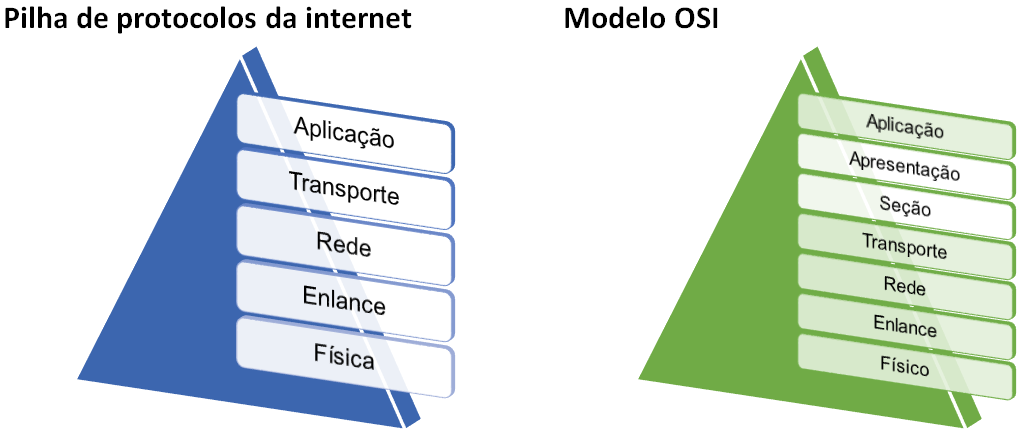
\includegraphics[width=0.9\textwidth]{figuras/osi_hierarquia.png}
	\caption{Comparação entre o modelo OSI e a pilha de protocolos da \emph{internet} (Próprio Autor).}
	\label{figura:osi_hierarquia}
\end{figure}

A camada com maior grau de abstração do TCP/IP é a aplicação. Nela contém os protocolos de nível de abstração mais elevados, responsáveis por oferecer os serviços à máquina ou usuário final. O SSH é um exemplo de protocolo desta camada que oferece o serviço de acesso remoto aos computadores. Outros serviços dessa camada são enviar arquivos (Protocolo FTP, BitTorrent), navegar na web (Protocolo HTTP) e comunicar-se através de chat (Protocolo IRC). Estes protocolos geralmente são implementados via software junto com a camada de transporte.

A camada de transporte é responsável por transportar as mensagens da camada de aplicação. Existem dois protocolos nesta camada, o TCP, que veio primeiro e também foi o responsável pelo acrônimo TCP/IP, e o UDP, que veio depois devido a necessidade de aumentar a velocidade de transmissão em aplicações em tempo real. É importante ressaltar que alguns protocolos da camada de aplicação foram feitos para ser usado sob o protocolo TCP ou protocolo UDP, ou ambos. A maioria dos protocolos de aplicação são definidos sob o protocolo TCP, como a navegação web (HTTP) e transferência de arquivos (FTP), outros são definidos apenas sob o protocolo UDP, como os protocolos de jogos online, vídeo conferência e voIP \footnote{Tecnologia de comunicação que utiliza o Internet Protocol para transferir chamadas telefônicas e serviços de voz de uma maneira geral.} (voice over IP).

A camada de rede é responsável por movimentar os pacotes de dados de uma máquina para outra. Esta camada tem dois componentes principais, o primeiro deles é o protocolo IP, que define o famoso conjunto de 4 números separados por pontos, os endereços de IP. O protocolo de IP é único e é ele quem caracteriza os sistemas que utilizam a pilha de protocolos TCP/IP. O outro componente da camada de rede são os protocolos de roteamento. Estes protocolos só fazem sentido em redes maiores, como as redes locais ou a rede mundial de computadores. Como, na nossa aplicação, estamos interessados apenas na comunicação ponto a ponto entre o computador e o BBB, utilizando a USB, esta segunda parte da camada de rede é irrelevante. Neste caso, o endereço de IP padrão do BeagleBone é $192.168.7.2$. O componente roteamento só se torna relevante se o BBB for conectado à rede local pela porta Ethernet (Item 10 da figura \ref{figura:bbb_components}), através de um roteador.

A camada de enlance de dados, que, por sua vez, significa, ligação ou \emph{link} de dados, define as especificações de transmissão, recepção, controle de fluxo, opcionalmente, a correção de erros que venham a ocorrer na camada física. As especificações desta camada estão intimamente ligadas ao meio em que se propagam. A família de protocolo DSL, por exemplo, é muito comum nas bandas largas comerciais, pois foi projetado para utilizar as linhas telefônicas como meio de transmissão. Já o protocolo Wi-Fi foi projetado para ser utilizado em redes locais cujo o meio de transmissão é o ar, assim é tem suporte a senhas de acesso, correção de erro e tem um limite de usuários simultâneos menor do que protocolos para redes sem fio maiores, como o LTE, padrão utilizado na \emph{internet} móvel dos celulares. Nas redes locais com fio é comum utilizar o protocolo Ethernet na camada de enlace.

\begin{figure}[h]
	\centering
	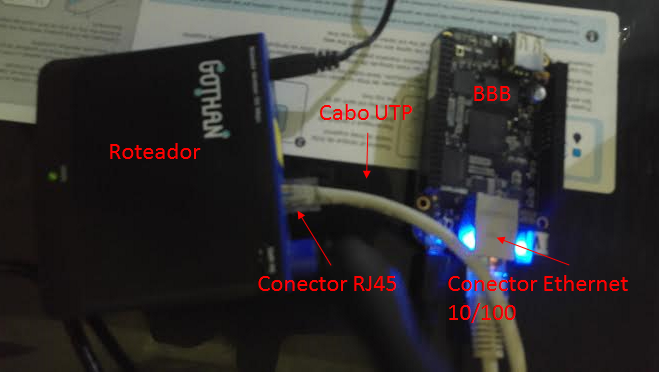
\includegraphics[width=\textwidth]{figuras/bbb_roteador.png}
	\caption{BeagleBone Black conectado a um roteador (Próprio Autor)}
	\label{figura:bbb_roteador}
\end{figure}

A camada física é o próprio meio de transmissão, ou seja, o ar, cabo coaxial, linhas telefônicas. Como dito anteriormente, é comum que os padrões da camada de enlance seja implementado em conjunto com a camada física, por isso, os circuitos integrados de rede geralmente já implementam as três camadas mais básicas (Rede, enlance e físico) via \emph{hardware}. Por exemplo, as placas de rede dos computadores pessoais especificam que deve ser utilizado como camada física cabos UTP com conectores RJ45 em conjunto com o protocolo Ethernet na camada de enlance e o protocolo IP na camada de rede. O CI SMSC do BeagleBone (Item 6 da figura \ref{figura:bbb_components}) segue esta mesma especificação e é utilizado em conjunto com o conector Ethernet 10/100 (Item 10 da figura \ref{figura:bbb_components}). Neste caso o BeagleBone deve ser conectado a um roteador como mostra na figura \ref{figura:bbb_roteador}. Como não estamos utilizando a porta USB, o endereço de IP da placa de desenvolvimento será diferente de $192.168.7.2$.

Um outro cenário possível é a utilização do protocolo Ethernet sobre a porta USB (Ethernet \emph{over} USB).  A porta USB é bastante utilizada para conectar periféricos a computadores e muitas vezes estes periféricos deve utilizar protocolos definidos para funcionar exclusivamente sobre IP, por isso, é comum que impressoras, celulares, \emph{smartphones} e dispositivos embarcados que utilizam a porta USB para se comunicar com o computador, implementem as camadas de enlance e rede via \emph{software} para que seja possível utilizar os serviços disponibilizados por IP. 

No caso de dispositivos embarcados com Linux isso é quase uma obrigação, visto que o próprio Linux já vem com driver USB-eth, que implementa os protocolos Ethernet e IP sobre a interface física da USB, criando uma rede local entre cliente e hospedeiro, no nosso caso computador e BeagleBone. A partir daí quase todos os serviços e protocolos disponibilizados por IP estão possíveis, incluindo aí a comunicação remota via SSH. No Windows é importante que os drivers disponibilizados em \cite{bbbgettinstarted} estejam atualizados, pois ambos os lados (Computador e Beaglebone Black) devem estar preparados para este tipo de conexão. 

Pelo fato do protocolo Ethernet não ser um padrão definido na comunicação USB, e ainda ser implementado via \emph{software}, é normal que o desempenho teórico fique abaixo dos $480Mbps$ teórico da USB 2.0. Segundo o usuário \emph{jons34yp} do site de perguntas e respostas, superuser.com \cite{usbethernetspeed}, foi possível atingir a média de $90Mbps$ em uma comunicação entre um smartphone com Android e um computador.  Para este trabalho taxas de transferências próximas a $1Mbps$ são mais do que o suficiente.

Voltando a falar sobre SSH, o Linux, Mac e sistemas operacionais baseados no Unix, já vem com suporte nativo a SSH, que pode ser acessado através do terminal. Entretanto, usuários do Windows devem baixar um cliente SSH como o PuTTY (Disponível em: \emph{http://www.putty.org/}). Antes de iniciar o processo de comunicação é importante atualizar os \emph{drivers} disponivel em: \emph{http://beagleboard.org/static/beaglebone/latest/README.htm}. Depois da atualização feita e o PuTTY baixado abra este aplicativo e no campo \emph{Host Name (or IP address)} escreva o IP do BeagleBone que por padrão é $192.168.7.2$. Deixe as outras opções padrões como mostra a figura \ref{figura:putty_interface}. Por fim, clique em Open para iniciar uma conexão SSH entre o computador e o Beaglebone Black. Uma janela de terminal se abrirá, inicialmente, pedindo para que o usuário entre com um \emph{login} e senha. Mais detalhes de como operar o terminal do Beaglebone Black pode ser visto na seção \ref{ch:bbb_terminal}.

\begin{figure}[h]
	\centering
	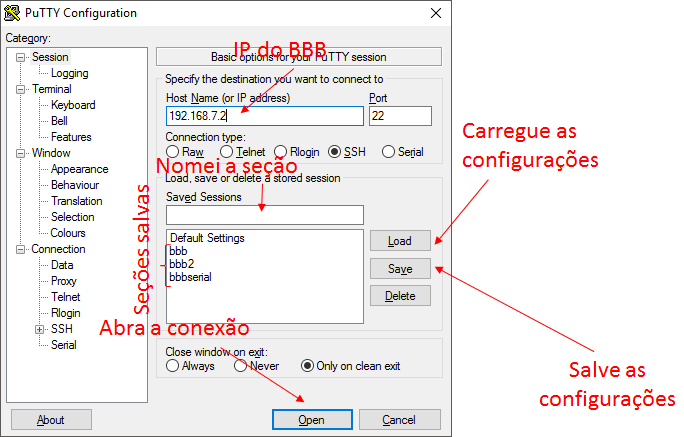
\includegraphics[width=\textwidth]{figuras/putty_interface.png}
	\caption{Configurações para conectar o BBB com o computador através do PuTTy (Próprio Autor)}
	\label{figura:putty_interface}
\end{figure}

Existe a possibilidade de criar configurações predefinidas neste aplicativo. Para isso, preencha os campos e selecione as opções de acordo com o desejado. Depois, no campo \emph{Saved Secctions} escreve o nome desta configuração e clique em \emph{Save}. Caso o usuário, por algum motivo, feche o PuTTY e abra-o novamente os campos do aplicativo serão restaurados para os seus valores padrões. Se houver alguma configuração pre-definida é possível carregá-la rapidamente apertando o botão \emph{Load}.

\begin{figure}[h]
	\centering
	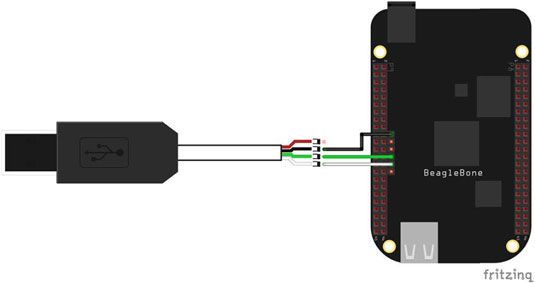
\includegraphics[width=\textwidth]{figuras/bbb_ttl.jpg}
	\caption{Conectando o UART0 do Beaglebone Black ao computador (Próprio Autor)}
	\label{figura:bbb_ttl}
\end{figure}

\subsection{Terminal no BeagleBone Black}
\label{ch:bbb_terminal}

Na seção \emph{

\subsection{Programando no BeagleBone Black}
\label{ch:bbb_programming}

O fato do BeagleBone Black utilizar Linux como sistema operacional o usuário programe em uma infinidade de linguagens de programação, entretanto algumas delas necessitam de passos adicionais. Esta que não vêm instaladas por padrão não serão abordadas nesta seção.

Ao conectar o Beaglebone Black ao computador através da porta USB Client (Item 14 na figura\ref{figura:bbb_components}) será montada a partição FAT \emph{BeagleBone Getting Star


Nas seções anteriores vimos os componentes do BBB e 

Como foi dito na seção \

O fato do BBB já vim com o linux embarcado permite que possa programar em 